\documentclass[aspectratio=169]{beamer}
\usepackage{hyperref}
\usepackage{listings}
\usepackage{tkz-berge}
\setbeamertemplate{caption}[numbered]

% \usepackage{fontspec}
% \setmonofont{Consolas}

\definecolor{background}{RGB}{39, 40, 34}
\definecolor{string}{RGB}{230, 219, 116}
\definecolor{comment}{RGB}{117, 113, 94}
\definecolor{normal}{RGB}{248, 248, 242}
\definecolor{identifier}{RGB}{166, 226, 46}
\definecolor{keyword}{HTML}{F92672}
\definecolor{numbers}{HTML}{AE81FF}
\definecolor{types}{HTML}{66D9EF}


\lstset{
    language=C++,
    tabsize=4, % tab space width
    showstringspaces=false, % don't mark spaces in strings
    numbers=left, % display line numbers on the left
    basicstyle=\ttfamily,
    numberstyle=\color{comment}\ttfamily, % Line numbers
    commentstyle=\color{comment}\ttfamily, % comment color
    otherkeywords={>,<,-,!,=,~}, % Color operators too
    morekeywords={>,<,-,!,=,~},
    keywordstyle=\color{keyword}\ttfamily, % keyword color
    stringstyle=\color{string}\ttfamily, % string color
    morecomment=[l][\color{keyword}]{\#},
    emph={int,char,long,float,double,unsigned,namespace,typename},
    emphstyle={\color{types}\ttfamily\textit},
    escapeinside={@!}{!@},
    captionpos=b
}
\newcommand{\code}{\texttt}
\newcommand{\fn}{\color{identifier}}
\renewcommand*{\thefootnote}{\fnsymbol{footnote}}
\usetheme{Warsaw}

\addtobeamertemplate{footnote}{\vspace{-6pt}\advance\hsize-0.5cm}{\vspace{6pt}}
\makeatletter
% Alternative A: footnote rule
\renewcommand*{\footnoterule}{\kern -3pt \hrule \@width 2in \kern 8.6pt}
% Alternative B: no footnote rule
% \renewcommand*{\footnoterule}{\kern 6pt}
\makeatother

\setbeamercolor{normal text}{fg=normal,bg=background}
\setbeamercolor{structure}{fg=normal}

\setbeamercolor{alerted text}{fg=red!85!black}

\setbeamercolor{item projected}{use=item,fg=background,bg=item.fg!35}

\setbeamercolor*{palette primary}{use=structure,fg=structure.fg}
\setbeamercolor*{palette secondary}{use=structure,fg=structure.fg!95!black}
\setbeamercolor*{palette tertiary}{use=structure,fg=structure.fg!90!black}
\setbeamercolor*{palette quaternary}{use=structure,fg=structure.fg!95!black,bg=black!80}

\setbeamercolor*{framesubtitle}{fg=normal}

\setbeamercolor*{block title}{parent=structure,bg=background}
\setbeamercolor*{block body}{fg=black,bg=background}
\setbeamercolor*{block title alerted}{parent=alerted text,bg=background}
\setbeamercolor*{block title example}{parent=example text,bg=background}

\title{Interview Skills}
\subtitle{Graph Algorithms}
\author{Richard Morrill}
\institute{Fordham University CS Society}
\logo{
\includegraphics[width=2cm]{css_logo_color.png}}
\date{Wednesday, January 9th 2019}

\section{}
\begin{document}
\begin{frame}
\titlepage
\end{frame}


\begin{frame}
    \frametitle{What is a Graph?}
    \pause
    \begin{figure}
    \begin{minipage}[c]{0.4\textwidth}
            \centering
            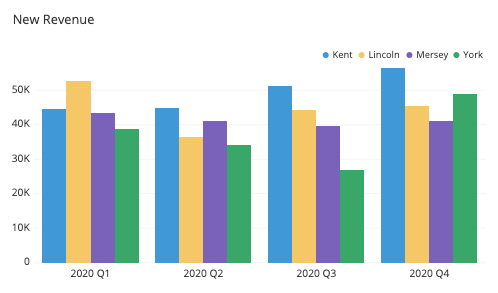
\includegraphics{bar_chart_example.png}
            \caption{Not This Kind of Graph!}
            \label{bargraph}
    \end{minipage}
    \hfill
    \pause
    \begin{minipage}[c]{0.4\textwidth}
            \centering
            \begin{tikzpicture}[draw=white,color=white]

                \tikzset{vertex/.style = {shape=circle,draw,minimum size=1.5em}}
                \tikzset{edge/.style = {->,> = latex'}}
                \node[vertex] (a1) at (0,0) {a1};
                \node[vertex] (a2) at (0,2) {a2};
                \node[vertex] (a3) at (2,0) {a3};
                \node[vertex] (a4) at (2,2) {a4};

                \draw[edge] (a1) to (a2);
                \draw[edge] (a1) to[bend left] (a4);
                \draw[edge] (a4) to[bend left] (a1);
                \draw[edge] (a2) to (a3);

            \end{tikzpicture}
            \caption{This Kind of Graph!}
            \label{fullyconnectedex}
        \end{minipage}
    \end{figure}
\end{frame}
\begin{frame}
    \frametitle{Characteristics of a Graph}
    \begin{itemize}
        \item Set of Nodes $S$
        \item Set of Edges $E \subset S^{2}$\footnote[frame]{This just means every possible ordered pair of nodes.}
        \pause
        \item Can represent a wide variety of real-world problems (such as?)
        \pause
        \begin{itemize}
            \item Islands \& Bridges
            \item Network Connections\only<3->\footnote[frame]{You'll see this come up when you take a networking class.}
            \item Intersections and Streets
        \end{itemize}
        \pause
        \item Position of nodes is for communication only
        \item Edges may have a ``weight'' assigned to them, which may represent distance in some cases
    \end{itemize}
\end{frame}
\begin{frame}
    \frametitle{Adjacency Matrix}
    \begin{itemize}
        \item Very useful for mathematical proofs
        \begin{figure}
            \begin{minipage}[c]{0.4\textwidth}
                \centering
                \begin{tikzpicture}[draw=white,color=white]

                    \tikzset{vertex/.style = {shape=circle,draw,minimum size=1.5em}}
                    \tikzset{edge/.style = {->,> = latex'}}
                    \node[vertex] (a1) at (0,0) {a1};
                    \node[vertex] (a2) at (0,2) {a2};
                    \node[vertex] (a3) at (2,0) {a3};
                    \node[vertex] (a4) at (2,2) {a4};
    
                    \draw[edge] (a1) to (a2);
                    \draw[edge] (a1) to[bend left] (a4);
                    \draw[edge] (a4) to[bend left] (a1);
                    \draw[edge] (a2) to (a3);
                    \draw[edge] (a1) to [loop below] (a1);
    
                \end{tikzpicture}
                \caption{Visual Representation of a Graph}
                \label{visgrap}
            \end{minipage}
            \hfill
            \begin{minipage}[c]{0.4\textwidth}
                \centering
                $\begin{pmatrix}
                    1 & 1 & 0 & 1 \\
                    0 & 1 & 0 & 0 \\
                    0 & 0 & 0 & 0 \\
                    1 & 0 & 0 & 0
                \end{pmatrix}$
                \caption{The Same Graph as \ref{visgrap}, in an Adjacency Matrix}
                \label{}
            \end{minipage}
        \end{figure}
        \pause
        \item Memory usage causes issues when used in programs.
    \end{itemize}
\end{frame}
\begin{frame}
    \frametitle{Representations of Graphs in Code}
    \begin{itemize}
        \item A graph is an \textbf{abstract data type (ADT)}
        \pause
        \begin{itemize}
            \item The operations you can perform on a graph are consistently defined.
            \item The actual way data is stored may vary from implementation to implementation.
        \end{itemize}
        \pause
        \item For higher level problems, you might use a graph library that provides a consistent interface to access and manipulate graphs.
        \item For now, though, it's important to show you know how to actually work with low-level implementations.
        \pause
        \item Graphs are most often represented as:
        \begin{itemize}
            \item Node Lists
            \item Edge Lists
        \end{itemize}
    \end{itemize}
\end{frame}
\begin{frame}[fragile]
    \frametitle{Node List}
    \begin{columns}
        \begin{column}{0.5\textwidth}
            \begin{tikzpicture}[draw=white,color=white]

                \tikzset{vertex/.style = {shape=circle,draw,minimum size=1.5em}}
                \tikzset{edge/.style = {->,> = latex'}}
                \node[vertex] (0) at (0, 4) {0};
                \node[vertex] (1) at (3, 4) {1};
                \node[vertex] (2) at (0, 2) {1};
            \end{tikzpicture}
        \end{column}
        \begin{column}{0.5\textwidth}
            \begin{lstlisting}
vector<vector<int>> graph = {
    {0, 4},
    {2, 3, 0},
    {0, 4},
    {3, 1, 4},
    {2, 3}
};
            \end{lstlisting}
        \end{column}
    \end{columns}

\end{frame}
\end{document}